\documentclass[12pt, letterpaper]{article}

\usepackage[utf8]{inputenc}
\usepackage{mathtools}
\usepackage{amsfonts}
\usepackage{amsmath}
\usepackage{graphicx}
\usepackage[a4paper, total={6in, 9in}]{geometry}

\DeclarePairedDelimiter{\ceil}{\lceil}{\rceil}

\title{CSE 21 HW 8}
\author{Brian Masse}
\date{March 12, 2025}

\begin{document}

\maketitle
\newpage

\bf{ 1. Given n cords, each with an innie connector type and outie connector type, determine if it possinle to string them all together in such a wa so taht you can plug your outie USB into the innie power outlet. }

% MARK: Problem 1a
\-\ \newline
\-\ \it{ a) Describe how to create a graph out of this problem such that the solution to the problem involves finding a Hamiltonian path }

\begin{itemize}
\item \textnormal{This graph will be directed. Plugging cable A into cable B does not imply you can plug cable B into cable A}
\item \textnormal{The set of all verticies: V = the set of all cables}
\item \textnormal{An edge (v,w) exists if the cable v can be plugged into the cable w. (The outie connector of v = the innie connector of w.)}
\item \textnormal{Finding a Hamiltonian path from a cable with a USB innie connector to a cable with power outtie connector represents connecting cables from the phone to the wall outlet using every vertex (cable)} \newline

\textnormal{If there exists a Hamiltonian path you can determine that it is possible to connect your phone to the wall using every cable. } \newline

\textnormal{If there is not a Hamiltonian path you can determine that it is not possible to connect your phone to the wall using every cable. }

\end{itemize}


% MARK: Problem 1b
\-\ \newline \newline 
\-\ \it{ b) Describe how to create a graph out of this problem such that the solution to the problem involves finding an Eulerian path. }
\begin{itemize}
\item \textnormal{ This graph will be directed. If there is a cable with innie connect A and outie connector B does not imply there is a cable with innie connector B and outie connector A  }
\item \textnormal{ The set of all verticies: V = the set of all connection types  }
\item \textnormal{ An edge (v, w) exists if there is a cable with innie part v and outie part w. }
\item \textnormal{ Finding an Eulerian path from the USB vertex to the power outlet vertex represents connecting the phone to the wall outlet using every edge (cable) } \newline

\textnormal{ If there exists a Eulerian path you can determine that it is possible to connect your phone to the wall using every cable } \newline

\textnormal{ If there is not a Eulerian path you can determine that it is not possible to connect your phone to the wall using every cable. } \newline

\end{itemize}

% MARK: Problem 1c
\-\ \newline \newline 
\-\ \it{ c) Draw your graph model for parts a and b on the particular set of cables described. }

\-\ \newline
\-\ \it{ Graph for part a, using Hamiltonian Path to solve } \newline
\begin{center}
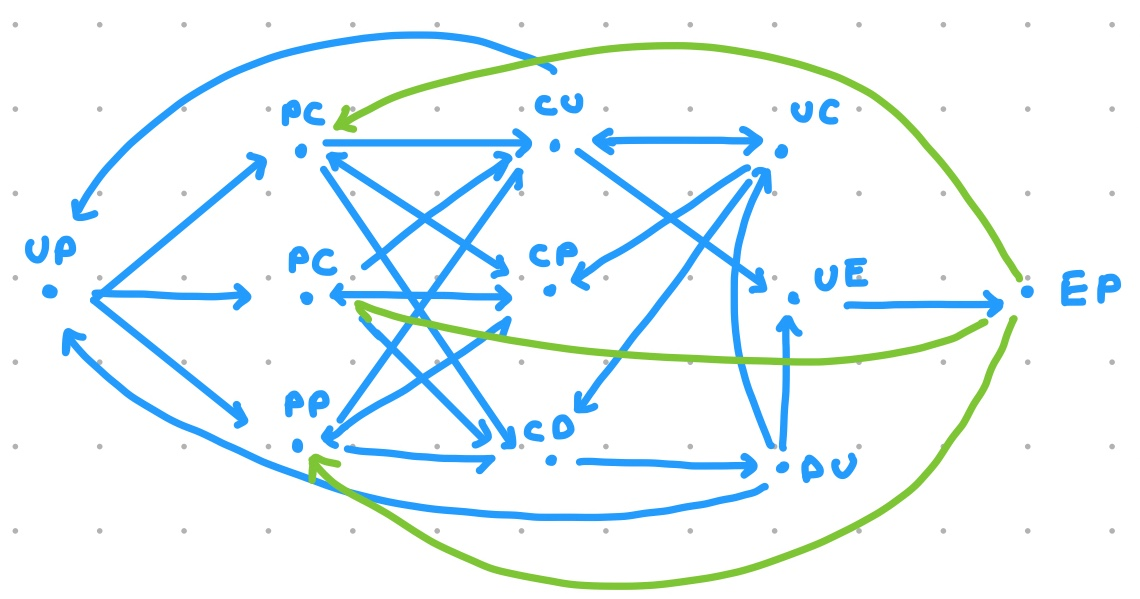
\includegraphics[width=0.85\textwidth]{graph1.jpeg}
\end{center}

\-\ \it{ Note: The first letter of a vertex is the innie connector, the second is the outtie connector }

\-\ \newline \newline
\-\ \it{ Graph for part b, using Eulerian Path to solve } \newline
\begin{center}
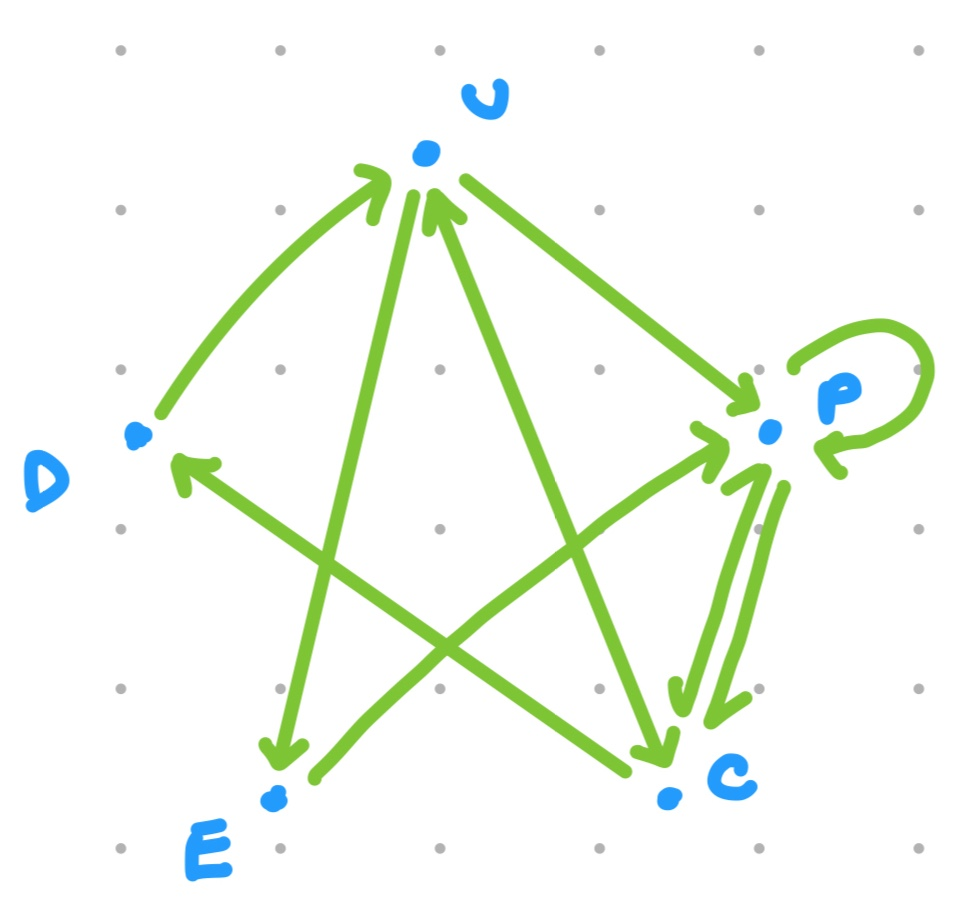
\includegraphics[width=0.5\textwidth]{graph2.jpeg}
\end{center}


\newpage

% MARK: Problem 2a
\bf{ 2. A binomial Tree is a special kind of rooted tree used for various data structures in computer science. A level d binomial tree cna be defined recursively. }

\-\ \newline

\-\ \it{ a) What is the hieght of a degree d binomial tree? Prove your result by induction on d. } 

\[ D(d) = 1 + D(d - 1); D(0) = 0\]
\[ D(d) = d \]

\begin{itemize}
  \item \textnormal{Base Case:} \newline  
  \textnormal{D(0) = 0. A single node has height 0.} \newline

  \item \textnormal{Induction Step. For some t \(>\) 0, assume D(t) = t. Show D(t) = t + 1} \newline
  \textnormal{D(t + 1) = 1 + D(t + 1 - 1) = t + 1}
\end{itemize}

% MARK: Problem 2b
\-\ \it{ b) Write a recurrence relation for the number of nodes N(d) in a binomial tree of degree d. }
\[ N(d) = 1 + \sum_{i = 1}^{n} N(d - i); N(0) = 1 \]

% MARK: Problem 2c
\-\ \it{ c) Use the guess-and-check method to guess a formula for N(d). Prove that your formula holds by induction on d. }

\[N(d) = \{1, 2, 4, 8, ...\}\]
\[ = 2^d \]

\textnormal{Proof by Induction:}
\begin{itemize}
  \item \textnormal{Base Case:} \newline
  N(0) = 1 = \(2^0\) = Number of nodes on a zero tree \newline

  \item \textnormal{ Induction Step (using Strong Induction): } \newline
  \textnormal{ \(\forall t > 0 \) assume \(N(t) = 2^t\). Show \(N(t + 1) = 2^{t + 1}\) } \\
  \begin{eqnarray*}
    N(t + 1) &=& 1 + N(t) + N(t - 1) + \dots \\
    &=& 1 + \sum_{i = 0}^{t} 2^i \\
    &=& 1 + \frac{s^{t + 1} - 1}{2 - 1} \\
    &=& 2^{t + 1}
  \end{eqnarray*}

\end{itemize}

% MARK: Problem 3
\newpage
\bf{ 3. Prove that for any integer \(n \ge 1\) any tournament graph on n verticies has a hamiltonian path. }

\begin{itemize}
\item \textnormal{ Base Case: } \newline
\textnormal{ If the tournament has 1 player then the graph with only 1 vertex has a trivial hamiltonian path. }

\item \textnormal{Inductive Step:} \newline
\textnormal{ Let n be an arbitrary integer such that \(n > 1\). Assume that for any tournament with n - 1 players, the corresponding graph has a hamiltonian path. } \newline \newline 
\textnormal{ Consider an arbitrary tournament T with n players \(\{1, ..., n\}\). Then if you consider the tournament T' involving only \{1,...n - 1\}, then by the inductive hypothesis, there is a hamiltonian path \((a_1,...,a_{n-1})\) in the corresponding graph. }

\begin{itemize}
\item \textnormal{Case 1: Player n wins against player \(a_1\). Then T has the hamiltonian path \((n, a_1,..., a_{n-1})\) }
\item \textnormal{Case 2: Player \(a_{n - 1}\) wins against player n. Then T has the hamiltonian path \((a_1,..., a_{n-1}, n)\) }
\item \textnormal{Case 3: Player n loses against player \(a_1\) and player n wins against player \(a_{n-1}\). Then T has the hamiltonian path \((a1, a2,..., a_{i - 1}, n, a_i,...a_{n-1} )\)} \newline \newline
\-\ \it{ Where \(a_i\) is the first in \((a_2,...a_{n-1})\) that n wins against.  }

\end{itemize}
\end{itemize}

\newpage
% MARK: Problem 4a
\bf{ 4. Recall that adjecncy matricies of simple direct graphos are matricies consisting of 0s and 1s such that there are no 1s down the diagonal. For the questions below suppose A is the adjency matrix of a simple directed graph G with n verticies. }

\-\ \newline
\-\ \it{ a) Consider the graph and its adjency matrix M. Compute \(M^2\) and \(M^3\) }

\[ M^2 = \begin{bmatrix}
  0 & 0 & 0 & 0 & 1 & 0 \\
  1 & 0 & 0 & 0 & 0 & 1 \\
  0 & 0 & 0 & 0 & 1 & 0 \\
  1 & 0 & 0 & 0 & 0 & 1 \\
  0 & 0 & 1 & 1 & 0 & 0 \\
  0 & 1 & 0 & 0 & 0 & 0
\end{bmatrix} \textnormal{  }
M^3 = \begin{bmatrix}
  1 & 0 & 0 & 0 & 0 & 1 \\
  0 & 0 & 1 & 1 & 0 & 0 \\
  1 & 0 & 0 & 0 & 0 & 1 \\
  0 & 0 & 1 & 1 & 0 & 0 \\
  0 & 1 & 0 & 0 & 1 & 0 \\
  0 & 0 & 0 & 0 & 1 & 0
\end{bmatrix}
\]

% MARK: Problem 4b
\-\ \newline
\-\ \it{b) Let A be an adjacency matrix of a simple directed graph. What does it mean to have non-zero entries in the diagonal of \(M^3\).}

\-\ \newline
\textnormal{If position \((i, i)\) in an adjacency matrix is non zero it means there is a circuit of length 3, starting and ending at vertex i. }


% MARK: Problem 4c
\-\ \newline
\-\ \it{c) Provide a justification for the following statement: Suppose that A is the adjacency matrix of a DAG. There exists some \(t \ge 2\) such that \(A^t\) is the zero matrix. }

\-\ \newline
\textnormal{ If there are no cycles in the graph, then every path in the graph must be finite. Let L be the longest path in the graph. Then there are no length \(t > L\) paths between any two verticies. Thus the adjacency matrix will be the zero matrix.  }


\end{document}
